\chapter{Introduction}
\label{cha:introduction}

% Important: you have to switch to arabic numbering here!
\pagenumbering{arabic}


\section{Word Embedding}


Machine learning approaches for natural language processing have to represent the words of a language in a way such that Machine Learning modules may process them. This is especially important for text mining, where data mining modules analyze text corpora. 

Consider a corpus \gls{C} %  $C$
of interest containing documents and sentences. Traditional text mining analyses use the vector space representation \citep{SaltonWongEtAl1975}, where a word $w$ is represented by a sparse vector of the size   \gls{N} % $N$
of the vocabulary  \gls{D} % $D$
(usually $N\ge 100.000$), where all values are 0 except the entry for the actual word. This representation is also called \emph{One-hot representation}. This sparse representation, however, has no information on the semantic similarity of words.

Recently word representations have been developed which represent each word $w$ as a real vector of \gls{d} % $d$ 
(e.g. $d=100$) real numbers as proposed by \citep{CollobertWeston2008} and  \citep{MikolovSutskeverEtAl2013}. Generally, we call such a vector  
$\gls{vw}\in\Re^k$ % v(w)
a \emph{word embedding}. By using a large corpus in an unsupervised algorithm word representations may be derived such that words with similar syntax and semantics have representations with a small Euclidean distance. Hence the distances between word embeddings corresponds to the semantic similarity of underlying words. These embeddings may be visualized to show comunalities and differences between words, sentences and documents. Subsequently these word representations may be employed for further text mining analyses like \emph{opinion mining} \citep{SocherPerelyginEtAl2013}, Kim 2014, Tang et al. 2014) or \emph{semantic role labeling} \citep{ZhouXu2015} which benefit from this type of representation \citep{CollobertWestonEtAl2011}.

These algorithms are based on the very important assumption that if the contexts of two words are similar, their representations should be similar as well \citep{Harris1954}.
Consider a sentence (or document) $S_i$ in the corpus $C$ consisting of \gls{Li} %$L_i$ 
words $\gls{Si} = (w_{i,1},w_{i,2},\ldots,w_{i,L_i})$. %% S_i
Then the context  of a word $w_t$ may be defined the words in the neighborhood of $w_t$ in the sentence.
Figure \ref{fig:neighbouring_words} shows how neighboring words determine the sense of the word "bank" in a number of example sentences. So many actual text mining methods make use of the context of words to generate embeddings. 
\begin{figure}[H]
\centering
\begin{minipage}{1.0\textwidth}
 
	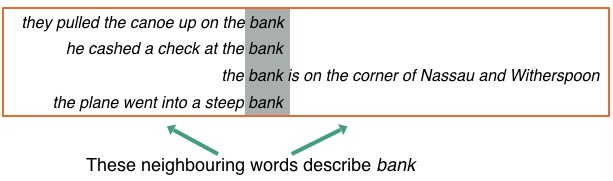
\includegraphics[width=1.0\textwidth]{neighbouring_words} 
	
\end{minipage}%
\label{fig:neighbouring_words}
\caption{Neigboring words defining the specific sense of "bank".}
\end{figure}	

Traditional word embedding methods first obtain the co-occurrence matrix and then perform dimension reduction suing singular value decomposition (SVD) ~ \citep{DeerwesterDumaisEtAl1990}. 

Recently, artificial neural networks is very popular to generate word embeddings. Prominent algorithms are \emph{Senna} \citep{CollobertWeston2008}, \emph{Word2vec} \citep{MikolovSutskeverEtAl2013} and Glove \citep{PenningtonSocherEtAl2014}. They all use randomly initialized vectors to represent words . Subsequently these embeddings are modified in such a way that the word embeddings of the neigboring words may be predicted with minimal error by a simple neural network function. 


\section{Sense Embedding}
Note that in the approaches described above each word is mapped to a single embedding vector. It is well known, however, that a word may have several different meanings, i.e. is \emph{polysemous}. For example the word "bank" among others may designate: 
\begin{itemize}
	\item the slope beside a body of water,
	\item a financial institution,
	\item a flight maneuver of an airplane.
\end{itemize}
Further examples of polysemy are the words "book", "milk" or "crane".
WordNet \citep{Fellbaum1998} and other lexical resources show, that most common words have 3 to 10 different meanings.
Obviously each of these meanings should be represented by a separate embedding vector, otherwise the embedding will no longer represent the underlying sense. This in addition will harm the performance of subsequent text mining analyses. Therefore we need methods to learn  embeddings for senses rather than words.


\emph{Sense embeddings} are a refinement of word embeddings. For example, "bank" can appear either together with "money", "account", "check" or in the context of "river", "water", "canoe". And the embeddings of "money", "account", "check" will be quite different from the embeddings of "river", "water", "canoe". Consider the following two sentences 
\begin{itemize}
	\item They pulled the canoe up the bank.
	\item He cashed a check at the bank.
\end{itemize}
The word "bank" in the first sentence has a different sense than the word "bank" in the second sentence. Obviously, the context is different. 

So if we have a methods to determine the difference of the context, we can relabel the word "bank" to the word senses "bank$_1$" or "bank$_2$" denoting the slope near a river or the financial institution respectively. We call the number after the word the sense labels of the word "bank". This process can be performed iteratively for each word in the corpus by evaluating its context.

An alternative representation of words is generated by topic models \citep{BleiNgEtAl2003}, which represent each word of a document as a finite mixture of topic vectors. The mixture weights of a word depend on the actual document. This implies that a word gets different representations depending on the context. 

In the last years a number of approaches to derive sense embeddings have been presented. \cite{HuangSocherEtAl2012} used the clustering of precomputed one-sense word embeddings and their neighborhood embeddings to define the different word senses. The resulting word senses are fixed to the corresponding word neighborhoods and their values are trained until convergence. A similar approach is described by \cite{ChenLiuEtAl2014}. Instead of a single embedding each word is represented by a number of different sense embeddings. During each iteration of the supervised training, for each position of the word, the best fitting embedding is selected according the fitness criterion. Subsequently only this embedding is trained using back-propagation. Note that during training a word may be assigned to different senses thus reflecting the training process. A related approach was proposed by \cite{TianDaiEtAl2014}.


\section{Goal}


It turned out that the resulting embeddings get better with the size of the training corpus and an increase of the dimension of the embedding vectors. This usually requires a parallel environment for the execution of the training of the embeddings. Recently \emph{Apache Spark} \citep{ZahariaChowdhuryEtAl2010} has been presented, an opensource cluster computing framework. Spark provides the facility to utilize entire clusters with implicit data parallelism and fault-tolerance against resource problems, e.g. memory shortage. The currently available sense embedding approaches are not ready to use compute clusters, e.g. by Apache Spark. 

Our goal is to investigate sense assignment models which will extend known word embedding (one sense) approaches and implement such method on a compute cluster using Apache Spark to be able to process larger training corpora and employ higher-dimensional sense embedding vectors. So that we can derive expressive word representations for different senses in an efficient way. And our main work will focus on the extension of Skip-gram model \citep{MikolovSutskeverEtAl2013} in connection to the approach of \citep{NeelakantanShankarEtAl2015} because these models are easy to use, very efficient and convenient to train. 


\section{Outline}

The rest of the report is structured as the following. Chapter 2 introduces the background about word embedding and explain the mathematical details of one model (word2vec \cite{MikolovSutskeverEtAl2013}) that one must be acquainted with in order to understand the work presented. Chapter 3 presents some relevant literatures and several latest approaches about sense embedding. Chapter 4 describes the mathematical model of our work for sense embedding. Chapter 5 introduces Spark framework and discusses in detail the implementation of our model. Chapter 6 analyzes the effect of different parameters from the model and compares the result with other models. Chapter 7 represents concluding remarks to our work including the advantages and disadvantages and talks about what can be done further to improve our model.
